\section*{Задача}
Реализовать программу, моделирующую выполнение протокола голосования для
12 файловых серверов при помощи пересылок MPI типа точка-точка. Получить
временную оценку времени выполнения одним процессом 3-х операций записи и
10 операций чтения $N$ байтов информации с файлом, расположенным (размноженным)
на 12 серверах. Определить оптимальные значения кворума чтения и кворума записи
для $N=300$. Время старта равно 100, время передачи байта равно 1
($Ts=100$,$Tb=1$).


\section*{Реализация}

Реализуем алгорим работы файловых серверов при помощи пересылок MPI типа
точка-точка. Это потребует небольшой модификации алгоритма, описанного на
лекциях и в книге Э.С.\,Таненбаума "Распределенные системы"\,, для корректной
обработке дедлоков без назначения тайм-аута, используя только передачи типа
точка-точка.

На рис. \ref{fig:all} приведена подробная блок-схема модифицированного
алгоритма. Подпрограмма "Получить все ответы"\, приведена на рис.
\ref{fig:get_all_req}.

Части хемы в большем масштабе приведены на рис. \ref{fig:read},
\ref{fig:write}, \ref{fig:idle}.

\begin{figure}[H]
    \centering
    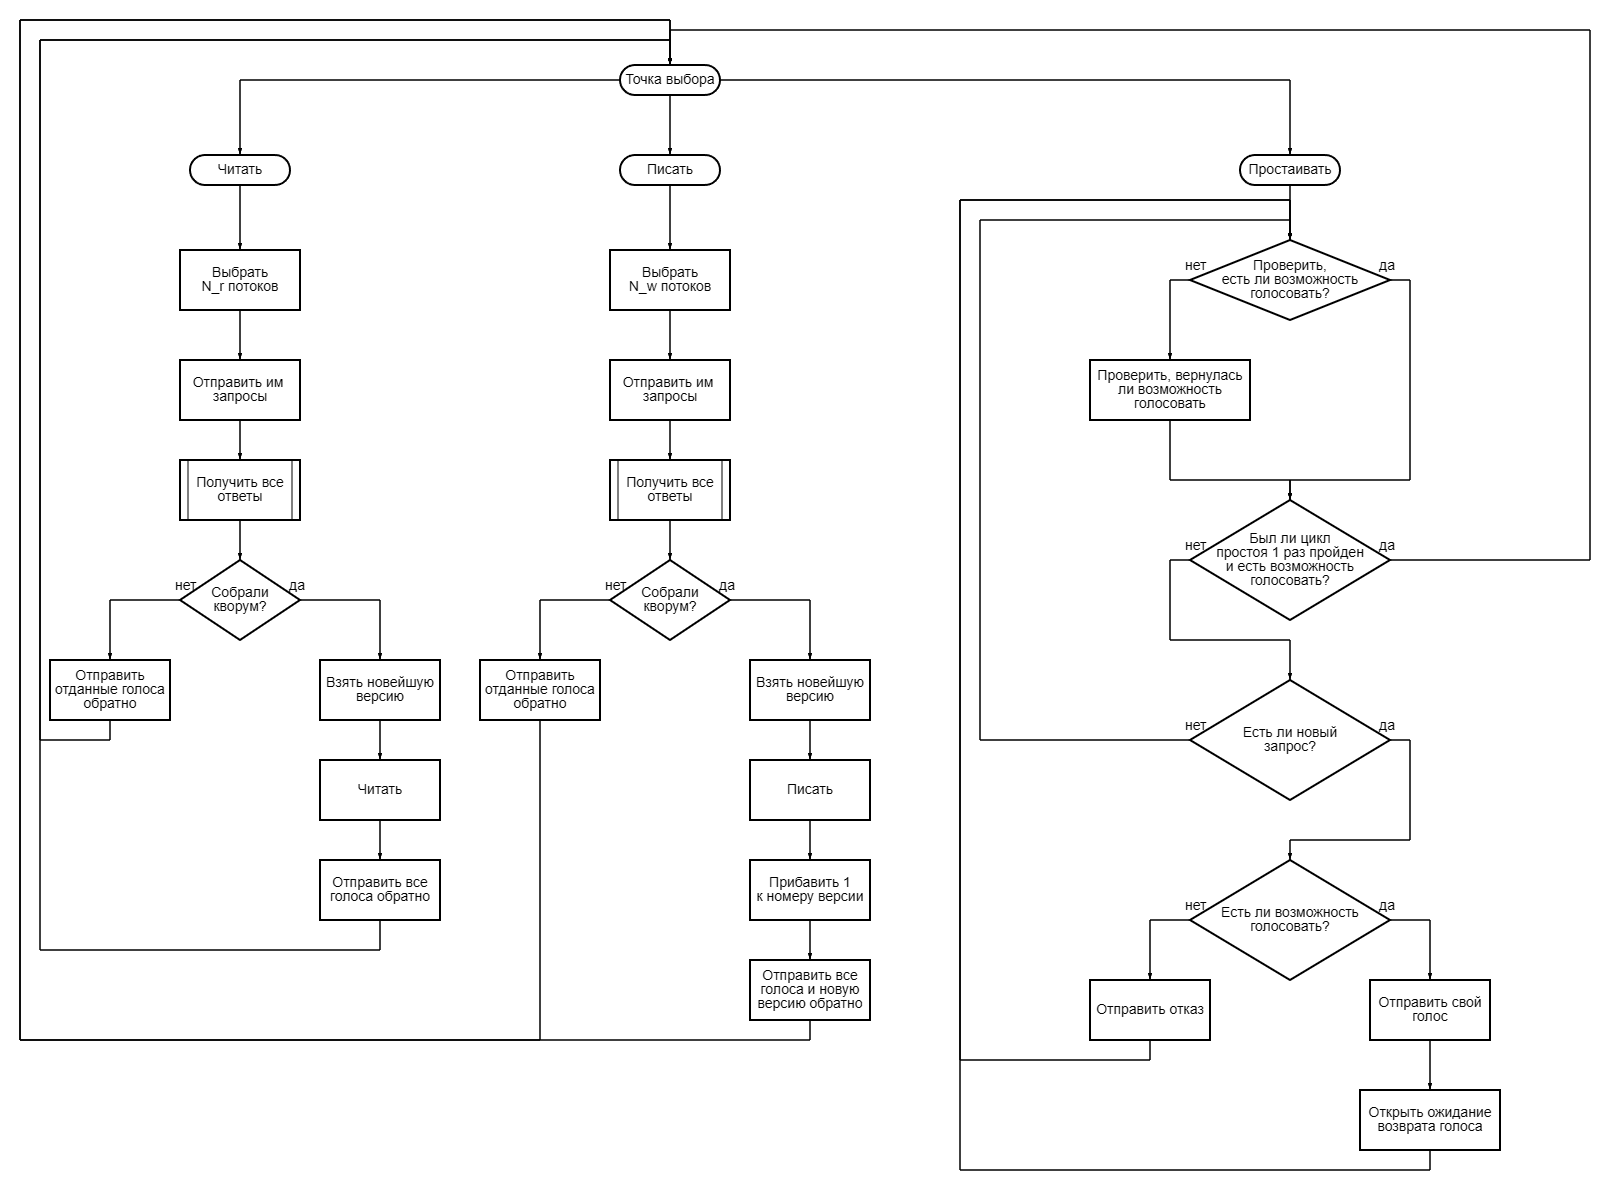
\includegraphics[width=1.1\linewidth,center]{all.png}
    \caption{Схема работы алгоритма}
    \label{fig:all}
\end{figure}

\begin{figure}[H]
    \centering
    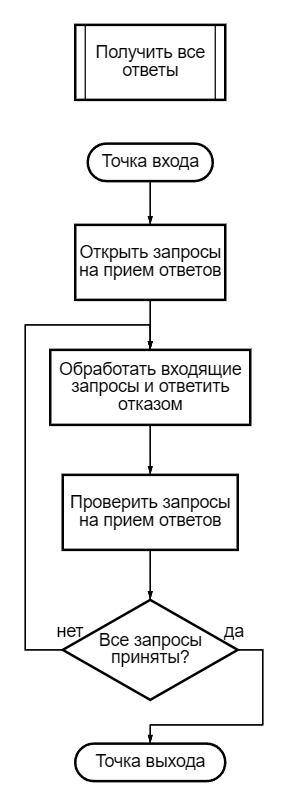
\includegraphics[width=.4\linewidth,center]{get_all_req.png}
    \caption{Подпрограмма "Получить все ответы"\,}
    \label{fig:get_all_req}
\end{figure}

Части схемы с рис. \ref{fig:all} в большем масштабе:

\begin{figure}[H]
    \centering
    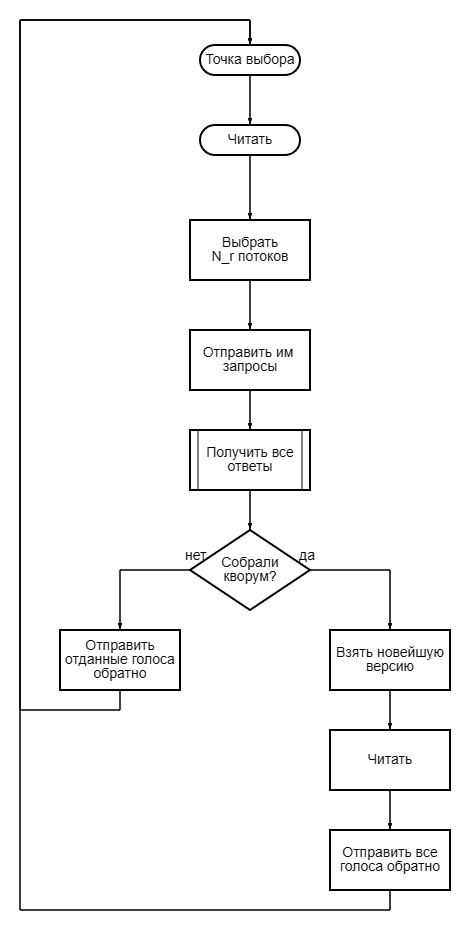
\includegraphics[width=.7\linewidth,center]{read.png}
    \caption{Схема чтения}
    \label{fig:read}
\end{figure}

\begin{figure}[H]
    \centering
    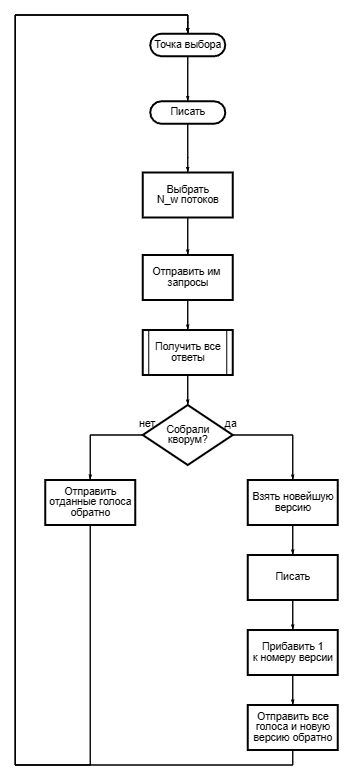
\includegraphics[width=.6\linewidth,center]{write.png}
    \caption{Схема записи}
    \label{fig:write}
\end{figure}

\begin{figure}[H]
    \centering
    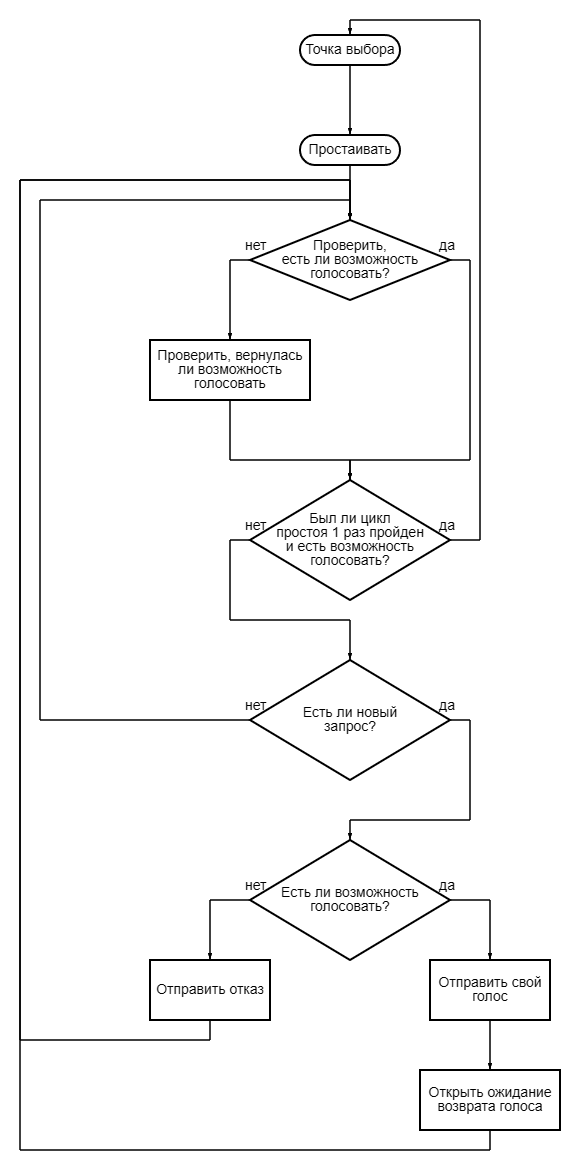
\includegraphics[width=.7\linewidth,center]{idle.png}
    \caption{Схема простаивания}
    \label{fig:idle}
\end{figure}



% \section{Ход работы}

% \textit{Ниже написан полнейший БРЕД (точнее компиляция лабораторных), чтобы показать, как делать то или иное действие в латехе и оверлифе. Все совпадения случайны.}

% Дана система с произвольной задержкой

% $\dot{x} = Ax(t) + A_1 x (t-h), $
% $A =
% \begin{bmatrix}
% 1 &  0\\
% 4 & 3\\
% \end{bmatrix},
% A_1 =
% \begin{bmatrix}
% -2 & 1 \\
% -2 & -6\\
% \end{bmatrix}$

% $\begin{bmatrix}
% \Phi & P - P_2^T (A+A_1)^T P_3 & -h P_2^T A_1\\
% * & -P_3 - P_3^T + hR & -h P_3^T A_1\\
% * & * & -hR\\
% \end{bmatrix} < 0,
% $

% $\Phi = P_2^T (A+A_1) + (A+A_1)^T P_2, P > 0, R > 0$

% Здесь $P_2$ и $P_3$ – произвольные матрицы. В результате решения матричного неравенства выше в MATLAB получена максимальная задержка $h = 0.18$, при которой система является устойчивой.

% Схема моделирования была собрана. Опытным путём удалось установить значение $K_{OC} = 2.5$ - максимальное допустимое, то есть значение при котором система устойчива (это граница устойчивости).

% \begin{figure}[H]
%     \centering
% \includegraphics[width=1.\linewidth,center]{scheme_1.png}
%     \caption{Схема моделирования}
%     \label{fig:my_label}
% \end{figure}

% % место для вывода про экстраполятор

% \subsection{Что-то там про колебательность}

% Колебательность процесса при фиксированном периоде квантования $T$ зависит от $K_{OC}$ следующим образом: чем больше $K_{OC}$ - тем больше система будет колебаться, пока не дойдёт до границы устойчивости, на которой она будет вести себя как чисто колебательная система без стремления к нулю.

% На графиках ниже можно видеть, как переходный процесс становится всё более колебательным и колебательным.

% Пусть степень устойчивости $\alpha = 0.5$. Тогда

% \begin{enumerate}
%     \item При $\mu = 3, \; \sigma(A+BK) = \{  -1.3192 \pm 5.2207i,  -0.9915, -1\}$
%     \item При $\mu = 1, \; \sigma(A+BK) = \{  -1.1340 \pm 5.5547i,  -0.9361, -1\}$
%     \item При $\mu = 0.4, \; \sigma(A+BK) = \{  -0.9402 \pm 5.8582i,  -0.7433, -1\}$
% \end{enumerate}


% \subsubsection{Графики}

% \begin{figure}[H]
%     \centering
% \includegraphics[width=1.\linewidth,center]{plot_y_2.png}
%     \caption{График $y(t)$ при $K_{OC} = 2$}
%     \label{fig:my_label}
% \end{figure}


% \begin{figure}[H]
%     \centering
% \includegraphics[width=1.\linewidth,center]{plot_y_23.png}
%     \caption{График $y(t)$ при $K_{OC} = 2.3$}
%     \label{fig:my_label}
% \end{figure}


% \begin{figure}[H]
%     \centering
% \includegraphics[width=1.\linewidth,center]{plot_y_25.png}
%     \caption{График $y(t)$ при $K_{OC} = 2.5$}
%     \label{fig:my_label}
% \end{figure}

% \begin{figure}[!htbp]
% \centering
% \begin{subfigure}{.5\textwidth}
%   \centering
%   \includegraphics[width=0.8\linewidth]{download (16).png}
%   \caption{Зелёные}
%   \label{fig:sub1}
% \end{subfigure}%
% \begin{subfigure}{.5\textwidth}
%   \centering
%   \includegraphics[width=0.8\linewidth]{download (17).png}
%   \caption{Оранжевые}
%   \label{fig:sub2}
% \end{subfigure}
% \label{fig:test}
% \caption{Сегментированные области}
% \end{figure}

% Максимальная колебательность наблюдается при $K_{OC} = 2.5$

% \subsubsection{Код Python}

% \begin{lstlisting}[language=Python, caption=Импорт и обычная бинаризация]
% import cv2
% from google.colab.patches import cv2_imshow
% from matplotlib import pyplot as plt
% import numpy as np
% from math import *
% import skimage
% from skimage import data, io, filters

% I=cv2.imread("pic.jpg",cv2.IMREAD_GRAYSCALE)
% cv2_imshow(I)
% t=127
% ret,Inew=cv2.threshold(I,t,255,cv2.THRESH_BINARY)
% plt.imshow(Inew)
% \end{lstlisting}
